\documentclass[a4paper]{article}
\usepackage{listings}
\usepackage{pgf}
\usepackage[utf8]{inputenc}
\usepackage{verbatim}
\usepackage{titling}
\usepackage{booktabs}
\usepackage{enumitem}
\usepackage{qtree}
\usepackage{amssymb}
\usepackage{amsmath}
\usepackage{times}
\usepackage{dsfont}
\usepackage{titling}
\usepackage[a4paper,
bindingoffset=0.2in,
left=1in,
right=1in,
top=2in,
bottom=1in,
footskip=.25in]{geometry}
\usepackage{cite} %bibtex
\usepackage{pdfpages}

\pretitle{\begin{center}\linespread{1}}
  \posttitle{\end{center}\vspace{0.14cm}} 
\preauthor{\begin{center}\Large}
  \postauthor{\end{center}}

\setlength{\droptitle}{-10em}
\title { \Large{Seminario de Ciencias de la Computaci\'on B}\protect\\
  \large{Heurísticas de Optimización Combinatoria}\protect\\
  \large{Problema del Ajente Viajero\\con Recocido Simulado}}


\date{\normalsize{Viernes, 17 de Marzo, 2023.}}
\author{\normalsize{Profesor: Canek Peláez Valdés}\protect\\
  \normalsize{Autor: Xin Wen Zhang Liu}}\vspace{0.2cm}

\clearpage



\begin{document}
\allowdisplaybreaks
\maketitle

\subsection*{El problema del agente viajero}
El problema del agente viajero es uno de los problemas de Optimización combinatoria m\'as estudiados. Introducido por primera vez en 1930 \\

Este problema plantea una pregunta f\'acil de hacer pero dif\'icil de repsonder:
\begin{center}
  Dado un conjunto de ciudades y sus coordenadas en el plano cartesiano, ?`cu\'al es el camino m\'as corto que visite cada ciudad exactamente una vez?
\end{center}
La manera m\'a directa de resolver este problema ser\'ia listar todas las prosibles combinaciones de caminos que pasen por las ciudades deseadas y comparar sus costos. Sin embargo el n\'umero de combinaciones diferentes con $n$ ciudades crece a la par de  $n!$, lo que hace que la cantidad de posibles combinaciones crezca a un paso colosal cuando incrementamos $n$.\\

Imaginemos que tenemos $5$ ciudades, entonces $5! = 5\times 4\times 3 \times 2\times 1 = 120$ , ahora dupliquemos el n\'umero de ciudades , entonces $10! = 10 \times 9 \dots \times 1 = 3,628,800$, podemos ver a esta cantidad crecer 

\subsection*{Recocido Simulado}
El  recocido simulado  (simulated annealing)  es un m\'etodo probabil\'istico propuesto por Kirkpatrick, Gelett y Vecchi (1983) y Cerny (1985) para encontrar el m\'inimo global de una funci\'on de costo que puede poseer m\'ultiples m\'inimos. Emulando el proceso f\'isico por el cual un s\'olido es lentamente enfriado para que al llegar a un estado de congelaci\'on, este lo haya hecho con una configuraci\'on de energ\'ia m\'inima.  ~\cite{sa}\\

Este m\'etodo se basa en obtener vecinos randomizados, donde se define una temperatura que decrementa lentamente, lo que nos da una cota superior que permite "subidas" que incrementan el costo, esperando que estas "subidas" lleven a un m\'inimo local. Esta proceso nos da una funcio\'
n que converge hacia la soluci\'on \'optima. 
\subsection*{Aceptaci\'on por umbrales}

\section*{Diseño}
El diseño de este programa usa el paradigma orientado a objetos, con una estructura bastante simple. Consiste de 5 clases structs
\begin{itemize}
\item  \texttt{Path} este struct contiene funciones de todas las operaciones que puedes realizar sobre estas. Este struct contiene como atributo igual una instancia de todas las ciudades guardadas en un vector, as\'i como
  \item \texttt{SimAnn}, como su nombre lo indica, este struct contiene los algoritmos del recocido simulado. Dentro de este, se encuentra la clase path como atributo
\item \texttt{TSI} este struct se encarga de generar hilos con instancias de \texttt{SimAnn}, para correr varias semillas al mismo tiempo, lo que facilita mucho la experimentaci\'on, ya que correr grupos de cualquier cantidad sin necesidad de atenci\'on constante del programador.

\end{itemize}
Adem\'as de estas estructuras 
\section*{Implementaci\'on}

El lenguaje usado para este proyecto fue Rust. Una de las cuantas razones fue la rapidez y su confiabilidad. La rapidez es un factor muy influyente en la experimentaci\'on, ya que facilita la r\'apida obtenci\'on de resultados para poder mejorar los par\'ametros usados.\\

Al comienzo del proyecto la principla dificultad fue el conocimiento del lenguaje. En la primera etapa del proyecto la inversi\'on de tiempo en comprender estructura, sintaxis y flujo de c\'odigo dentro de un nuevo lenguaje es un porcentaje bastante grande. 


\subsection*{El algoritmo}

\section*{Experimentaci\'on y resultados}
La etapa de la experimentaci\'on 

The higher the number of cities, a lower epsilon seems to work better. On the other hand for the case with 40 cities if the epsilo is 0.0001 then it seems to fall into a weird loop and the algorithm either doesn't end or take a long time  to finish. So it's not reaching the minimum temperature for some reason.

Also increasing 

\section*{Reproducir los resultados}
Una parte importante y la raz\'on por la que se usan semillas al generar los n\'umeros aleatorios, es que los resultados encontrados sean reproducibles.\\

Esta es la lista de variables usadas para obtener estos resultados, y c\'omo reproducirlos.

\subsection*{Para el caso con 40 ciudades}
Las variables usadas fueron
\begin{itemize}
\item Evaluaci\'on : 0.2637132755109184
\item El camino:
  \begin{align*}
    &[979, 493, 329, 163, 172, 496, 815, 657, 168, 1, 656, 2, 653, 490, 654, 7, 816, 982, 332, 820,\\
    &981, 333, 3, 165, 6, 5, 978, 817, 4, 489, 492, 491, 984, 331, 164, 327, 980, 186, 483, 54]
  \end{align*}
  
\item Epsilon : 0.002
\item Phi : 0.98
\item Tamaño de lote : 1000
\item Semilla de vecinos aleatorios : 16214040050592208640
\item Semilla para generar la soluci\'on inicial : 16042267250931732492
\end{itemize}
Para poder correr esta instancia, ejecutar lo siguiente desde la l\'inea de comandos.
\begin{lstlisting}
  cd target/release
  ./simulated_annealing --cities40 -e 0.002 --neigh 16214040050592208640
                        --init 16042267250931732492
\end{lstlisting}
% % (0.2637132755109184, [979, 493, 329, 163, 172, 496, 815, 657, 168, 1, 656, 2, 653, 490, 654, 7, 816, 982, 332, 820, 981, 333, 3, 165, 6, 5, 978, 817, 4, 489, 492, 491, 984, 331, 164, 327, 980, 186, 483, 54], 16214040050592208640, 16042267250931732492)
% 11613177925935108993, 8480295797754924014)
% % neighbor seed , initial_solution seed
\subsection*{Para el caso con 150 ciudades}
\begin{itemize}
\item Evaluaci\'on : 0.14418250861220022196
\item El camino:
  \begin{align*}
    &[54, 652, 1075, 483, 171, 77, 183, 346, 75, 821, 512, 179, 671, 16, 520, 186, 190, 675, 340, 502,\\
    &151, 828, 12, 1038, 339, 826, 444, 17, 164, 11, 501, 25, 492, 491, 499, 347, 489, 4, 174, 817,\\
    &23, 176, 668, 352, 978, 5, 6, 988, 165, 3, 981, 990, 333, 991, 351, 185, 22, 676, 665, 173, 2,\\
    &656, 184, 815, 172, 182, 496, 19, 505, 168, 508, 986, 9, 1, 829, 657, 663, 661, 832, 667, 507,\\
    &653, 344, 490, 654, 26, 820, 345, 332, 181, 14, 982, 187, 816, 678, 823, 7, 673, 163, 329, 509,\\
    &493, 979, 837, 995, 984, 1003, 349, 331, 662, 8, 999, 674, 334, 343, 510, 660, 20, 680, 825,\\
    &500, 985, 504, 511, 327, 670, 350, 840, 336, 297, 980, 191, 822, 1001, 74, 166, 658, 666, 818,\\
    &655, 819, 330, 1073, 169, 1037, 326, 328, 167, 495, 494]
  \end{align*}
  
\item Epsilon : 0.0001
\item Phi : 0.98
\item Tamaño de lote : 1000
\item Semilla de vecinos aleatorios : 11613177925935108993
\item Semilla para generar la soluci\'on inicial : 8480295797754924014
\end{itemize}
Primero se debe de cambiar la siguiete l\'inea de c\'odigo dentro del archivo \texttt{sa.rs}
\begin{lstlisting}
  105 let mut batch_average = 
\end{lstlisting}

despu\'es, ejecutar lo siguiente desde la l\'inea de comandos.
\begin{lstlisting}
  cd target/release
  ./simulated_annealing --cities150 --neigh 11613177925935108993
                        --init 8480295797754924014
                      \end{lstlisting}



%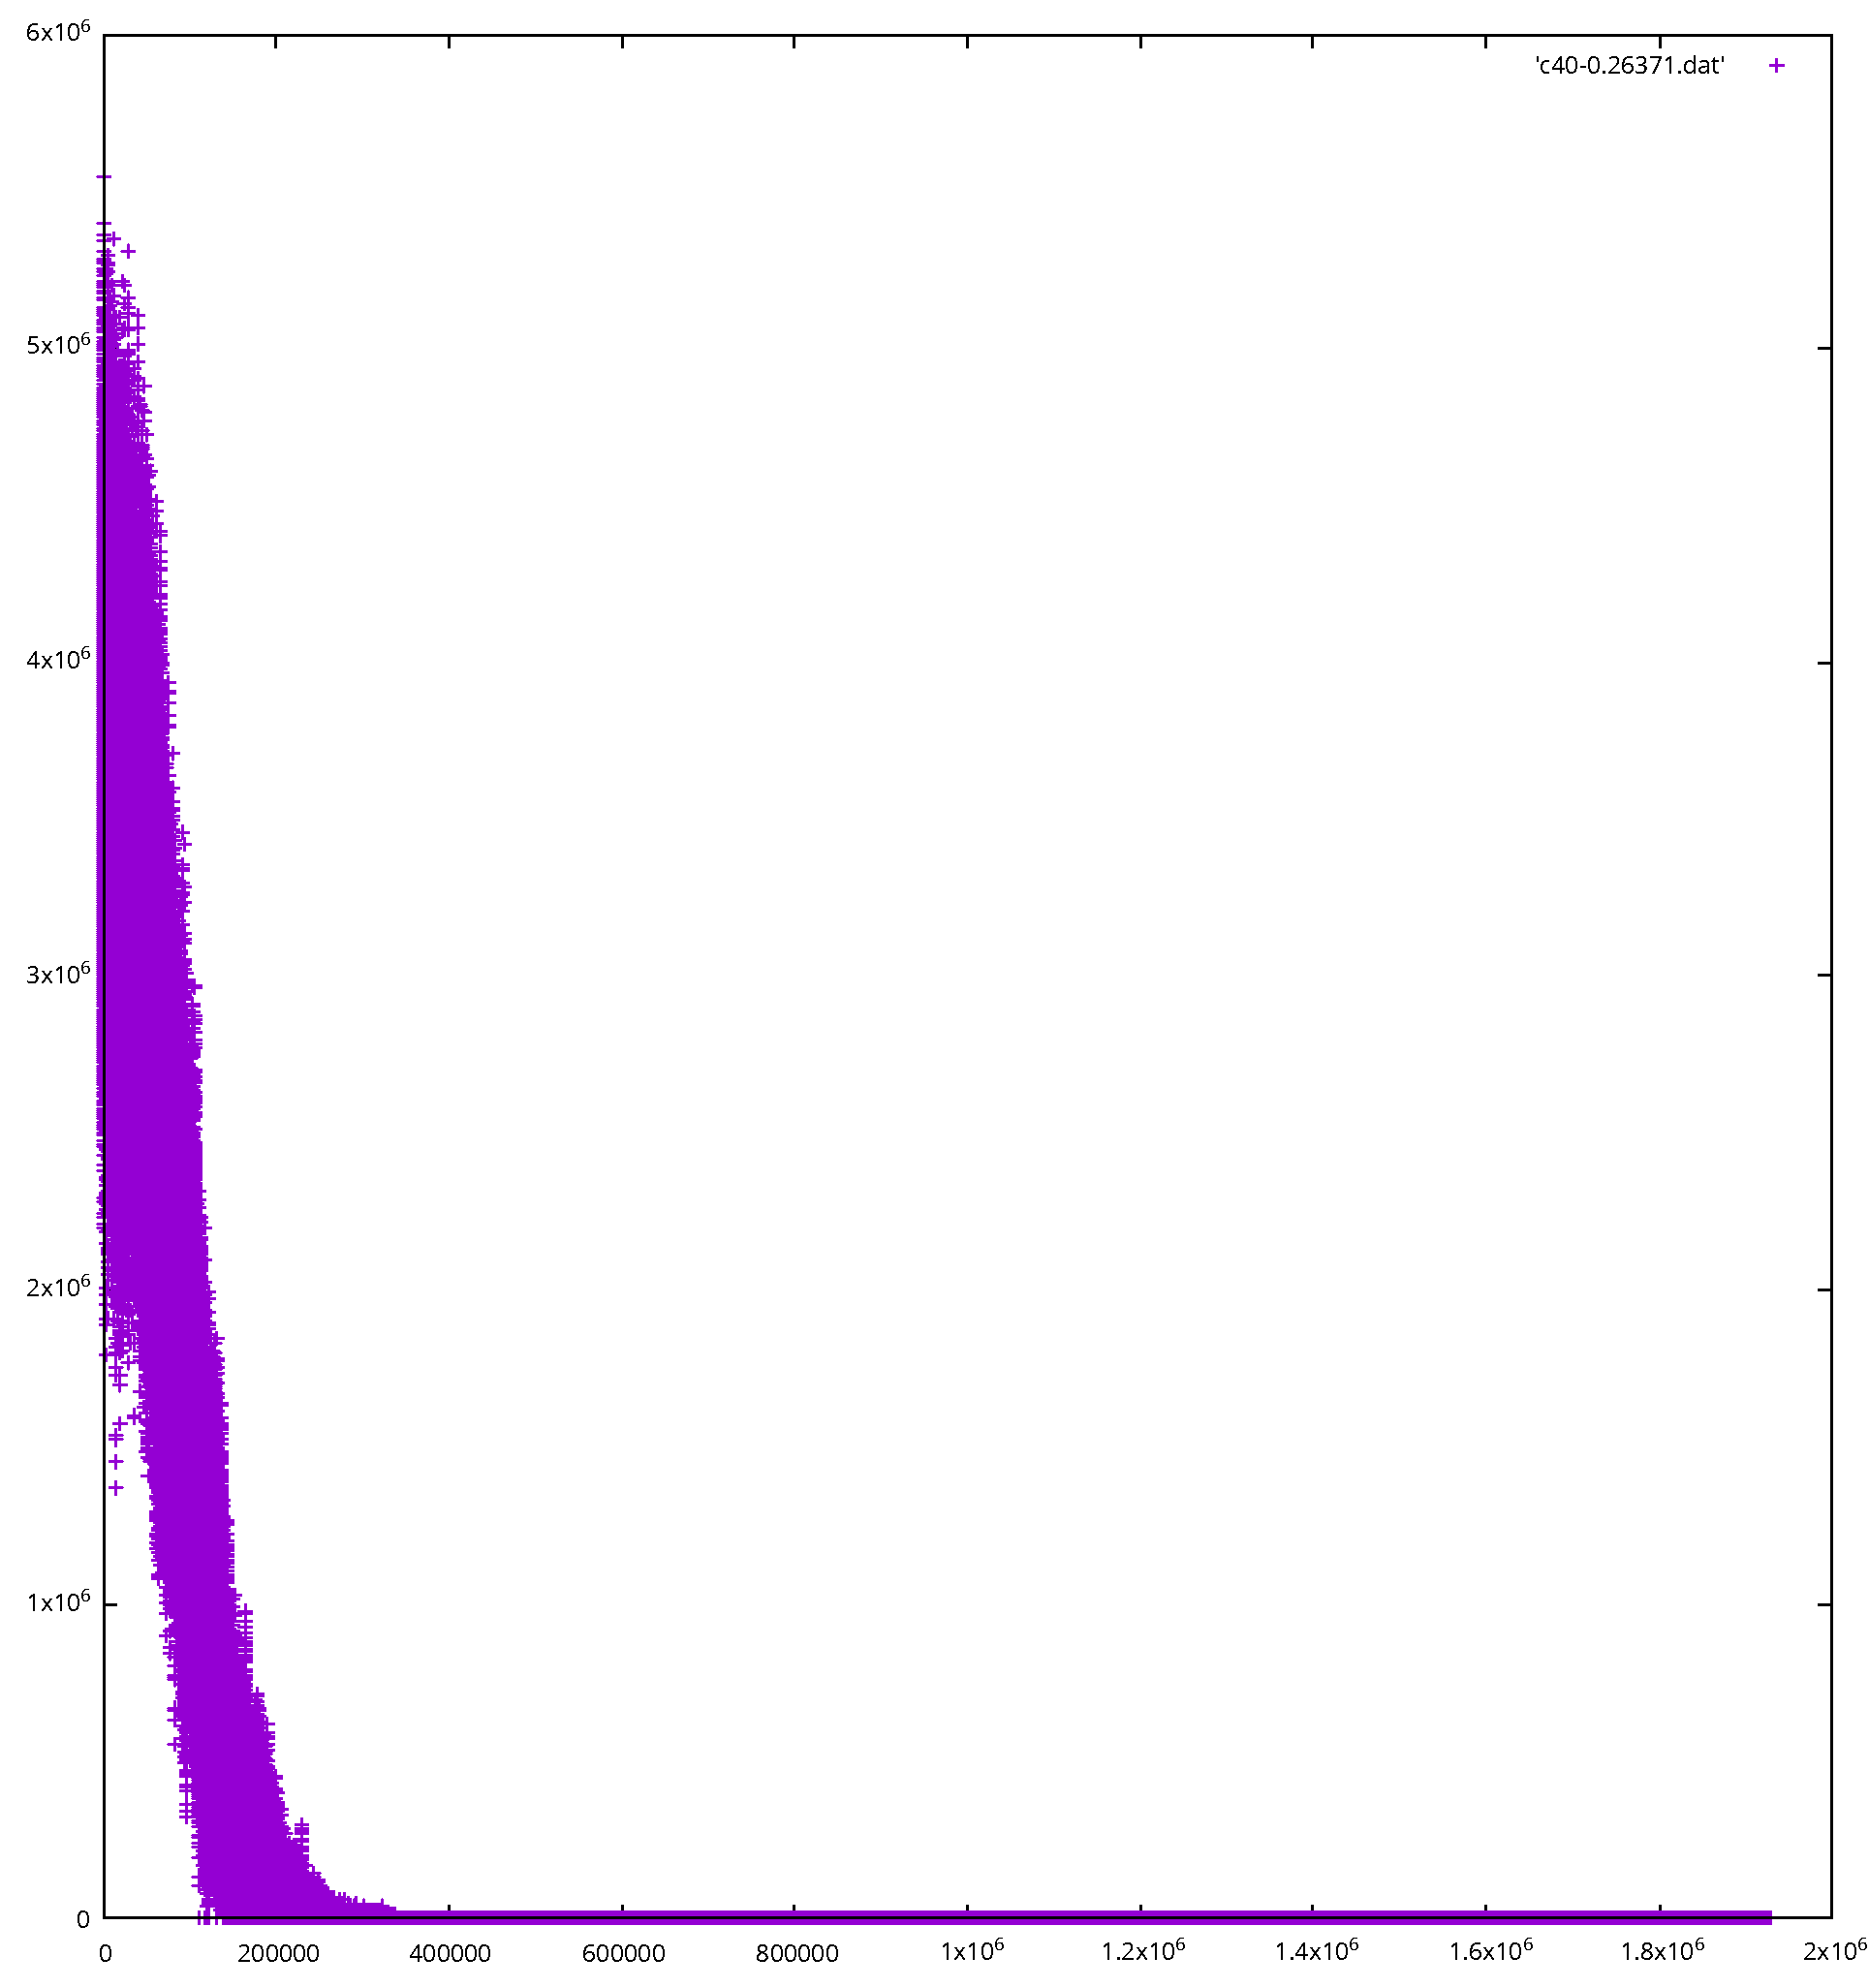
\includepdf[]{c40-0.26371.pdf}
\section*{Conclusiones}

\bibliography{citations}{}
\bibliographystyle{plain}
\end{document}